\documentclass[11pt,a4paper]{article}

\usepackage[top=20mm,bottom=26mm,left=20mm,right=20mm,headheight=15pt,footskip=12mm]{geometry}

\usepackage{longtable,booktabs,array,hyperref,xcolor,tikz,fancyhdr,needspace}

\usepackage{fontspec,xeCJK}

\setmainfont[Ligatures=TeXOff]{Times New Roman}

\setsansfont[Ligatures=TeXOff]{Times New Roman}

\setmonofont[Ligatures=TeXOff,WordSpace={1,1,1}]{Times New Roman}

\setCJKmainfont{Noto Serif CJK SC}

\setCJKsansfont{Noto Serif CJK SC}

\setCJKmonofont{Noto Serif CJK SC}

\newfontfamily\vulcanmathsymbols{Noto Serif CJK SC}

\XeTeXgenerateactualtext=1

\definecolor{vulcan}{HTML}{BB3E23}

\definecolor{vulcanblue}{HTML}{1B4F72}

\renewcommand{\thesection}{\Roman{section}}

\renewcommand{\thesubsection}{\Alph{subsection}}

\pgfdeclarelayer{connections}\pgfdeclarelayer{edge labels}\pgfsetlayers{connections,main,edge labels}

\hypersetup{hidelinks}

\newcolumntype{L}[1]{>{\raggedright\arraybackslash\hspace{0pt}}p{#1}}

\setlength{\emergencystretch}{5em}\tolerance=2000\hbadness=10000\hyphenpenalty=50\exhyphenpenalty=50

\setlength{\parindent}{0pt}\setlength{\parskip}{5pt}

\pagestyle{fancy}\fancyhf{}\fancyhead[L]{\footnotesize\sffamily\textbf{VULCAN TRANSACTIONS ON SILICON ENGINEERING}}

\fancyhead[R]{\footnotesize\sffamily RTL Microarchitecture \& Silicon Signoff}\fancyfoot[C]{\footnotesize\sffamily Page \thepage}

\begin{document}

{\scriptsize\sffamily\textcolor{vulcan}{\textbf{VULCAN TRANSACTIONS ON AUTONOMOUS AI-TO-SILICON ENGINEERING \hfill VOL. 2026 \textperiodcentered{} ARCHITECTURAL SIGNOFF PAPER}}\par}

\vspace{1pt}\textcolor{vulcan}{\rule{\textwidth}{1.2pt}}\vspace{4pt}

\begin{center}

{\sffamily\LARGE\bfseries SWAGE-S2 Programmable Streaming Image Processor\par}\vspace{3pt}

{\small\sffamily\textbf{Sufeng Guo (\allowbreak{}sufeng\_\allowbreak{}guo@smail.nju.edu.cn)\allowbreak{}} \textperiodcentered{} Microsoft Research Asia \textperiodcentered{} Technical Design and Verification Report\par}\vspace{1pt}

{\scriptsize\sffamily\textcolor{black!75}{Silicon Platform: Intel Arria 10 GX (\texttt{10AX115N3F40E2SG}) PCIe Gen3x8 \textperiodcentered{} Toolchain: Icarus Verilog 12.0 / Yosys 0.33 / Quartus Prime 17.1 STA \textperiodcentered{} 2 November 2026 (\allowbreak{}2026-11-02 19:57 UTC+\allowbreak{}8 Beijing Time)\allowbreak{}}\par}

\end{center}\vspace{2pt}

\renewcommand{\abstractname}{\textcolor{vulcanblue}{Abstract}}\begin{abstract}\noindent SWAGE-S2 extends the preserved SWAGE-S1 scaler with programmable signed 3x3 convolution and forward-2x2 RGGB demosaic. Frame-atomic configuration selects scaling alone or spatial processing followed by scaling. Separate three-line circular buffers avoid frame-sized storage. Software-vs-Hardware numerical comparison established bit-exact Python-reference parity with simulated RTL across 586 completed frames and 286,\allowbreak{}659 output pixels; 89,\allowbreak{}499 scale-only pixels were also compared with the unchanged parent. All seven deliberate RTL mutations were detected. L1 RTL timing lint passed. L2 Intel Quartus Prime 17.1 TimeQuest post-fit analysis achieved WNS\_\allowbreak{}setup =\allowbreak{} +\allowbreak{}5.206 ns at 100 MHz. L3 physical Arria 10 FPGA HIL passed three deterministic bridge-connectivity probes; it did not establish on-board image-processing numerical parity. [\allowbreak{}E021,\allowbreak{} E023–E025]\allowbreak{}\par\vspace{2pt}{\scriptsize\textbf{\textcolor{vulcanblue}{Index Terms---}}Autonomous RTL Generation, SystemVerilog, Intel Arria 10 GX FPGA, TimeQuest 100~MHz+ Timing Closure, PCIe Gen3x8 Hardware-in-the-Loop (HIL), Bit-Exact Fixed-Point Verification.}\end{abstract}\vspace{2pt}

\needspace{5\baselineskip}\section{Architecture and design rationale}

The single-clock swage\_\allowbreak{}s2\_\allowbreak{}top routes pixels through optional demosaic,\allowbreak{} optional convolution and the unchanged scaler. Spatial stages preserve source dimensions; scaling is always last. Configuration and three independent handshake counters prevent frame reuse until source admission,\allowbreak{} spatial-to-scaler transfer and destination retirement are complete. This explicitly handles downscaling that finishes destination output before the spatial tail drains. Each spatial window separates row filling from scanning,\allowbreak{} trading peak throughput for simple ownership and synchronous single-read memories. [\allowbreak{}E001,\allowbreak{} E008–E011]\allowbreak{}

\begin{center}\begin{minipage}{\textwidth}\centering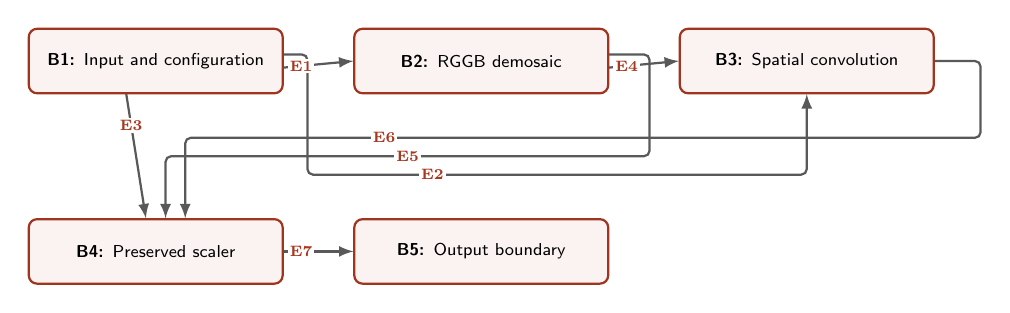
\begin{tikzpicture}[scale=0.78,transform shape,every node/.style={font=\footnotesize\sffamily},>=latex]

\node[draw=vulcan!85!black,thick,rounded corners=3pt,fill=vulcan!6,text width=3.9cm,minimum height=1.05cm,align=center] (b0) at (0.0,0.0) {\textbf{B1:} Input and configuration};

\node[draw=vulcan!85!black,thick,rounded corners=3pt,fill=vulcan!6,text width=3.9cm,minimum height=1.05cm,align=center] (b1) at (5.3,0.0) {\textbf{B2:} RGGB demosaic};

\node[draw=vulcan!85!black,thick,rounded corners=3pt,fill=vulcan!6,text width=3.9cm,minimum height=1.05cm,align=center] (b2) at (10.6,0.0) {\textbf{B3:} Spatial convolution};

\node[draw=vulcan!85!black,thick,rounded corners=3pt,fill=vulcan!6,text width=3.9cm,minimum height=1.05cm,align=center] (b3) at (0.0,-3.1) {\textbf{B4:} Preserved scaler};

\node[draw=vulcan!85!black,thick,rounded corners=3pt,fill=vulcan!6,text width=3.9cm,minimum height=1.05cm,align=center] (b4) at (5.3,-3.1) {\textbf{B5:} Output boundary};

\begin{pgfonlayer}{connections}

\draw[->,thick,black!65] ([yshift=-0.107cm]b0.east) -- coordinate[pos=0.25] (e0) ([yshift=0.000cm]b1.west);

\draw[->,thick,black!65,rounded corners=2pt] ([yshift=0.107cm]b0.east) -- (2.470,0.107) -- (2.470,-1.850) -- coordinate[pos=0.25] (e1) (10.600,-1.850) -- ([xshift=0.000cm]b2.south);

\draw[->,thick,black!65] ([xshift=-0.480cm]b0.south) -- coordinate[pos=0.25] (e2) ([xshift=-0.160cm]b3.north);

\draw[->,thick,black!65] ([yshift=-0.107cm]b1.east) -- coordinate[pos=0.25] (e3) ([yshift=0.000cm]b2.west);

\draw[->,thick,black!65,rounded corners=2pt] ([yshift=0.107cm]b1.east) -- (8.040,0.107) -- (8.040,-1.550) -- coordinate[pos=0.50] (e4) (0.160,-1.550) -- ([xshift=0.160cm]b3.north);

\draw[->,thick,black!65,rounded corners=2pt] ([yshift=0.000cm]b2.east) -- (13.430,0.000) -- (13.430,-1.250) -- coordinate[pos=0.75] (e5) (0.480,-1.250) -- ([xshift=0.480cm]b3.north);

\draw[->,thick,black!65] ([yshift=0.000cm]b3.east) -- coordinate[pos=0.25] (e6) ([yshift=0.000cm]b4.west);

\end{pgfonlayer}

\begin{pgfonlayer}{edge labels}

\node[fill=white,inner sep=1pt,font=\scriptsize\bfseries,text=vulcan!90!black] at (e0) {E1};

\node[fill=white,inner sep=1pt,font=\scriptsize\bfseries,text=vulcan!90!black] at (e1) {E2};

\node[fill=white,inner sep=1pt,font=\scriptsize\bfseries,text=vulcan!90!black] at (e2) {E3};

\node[fill=white,inner sep=1pt,font=\scriptsize\bfseries,text=vulcan!90!black] at (e3) {E4};

\node[fill=white,inner sep=1pt,font=\scriptsize\bfseries,text=vulcan!90!black] at (e4) {E5};

\node[fill=white,inner sep=1pt,font=\scriptsize\bfseries,text=vulcan!90!black] at (e5) {E6};

\node[fill=white,inner sep=1pt,font=\scriptsize\bfseries,text=vulcan!90!black] at (e6) {E7};

\end{pgfonlayer}

\end{tikzpicture}\par\vspace{3pt}

{\small\textbf{Figure 1:} Top-level microarchitectural functional block map and directed inter-module bus topology.}\end{minipage}\end{center}

{\small\renewcommand{\arraystretch}{1.18}\begin{longtable}{@{}L{0.24\textwidth}|L{0.7\textwidth}@{}}\toprule

\textbf{Block} & \textbf{Responsibility}\\\midrule\endhead

B1: Input and configuration & Admits one frame at a time,\allowbreak{} validates configuration,\allowbreak{} freezes controls during processing and selects active or bypass routes.\\[2pt]\hline

B2: RGGB demosaic & u\_\allowbreak{}demosaic contains an 8-bit u\_\allowbreak{}window and two registered arithmetic stages producing packed RGB from forward-2x2 samples.\\[2pt]\hline

B3: Spatial convolution & u\_\allowbreak{}convolution contains a packed-pixel u\_\allowbreak{}window and nine arithmetic stages for signed correlation,\allowbreak{} rounding,\allowbreak{} optional magnitude and saturation.\\[2pt]\hline

B4: Preserved scaler & u\_\allowbreak{}scaler is swage\_\allowbreak{}s1\_\allowbreak{}top,\allowbreak{} retaining u\_\allowbreak{}phase,\allowbreak{} u\_\allowbreak{}scheduler,\allowbreak{} u\_\allowbreak{}line\_\allowbreak{}buffer and u\_\allowbreak{}interp,\allowbreak{} including its six-stage interpolation pipeline.\\[2pt]\hline

B5: Output boundary & Presents destination pixels and aligned frame markers; downstream readiness propagates backward through the selected chain.\\[2pt]\hline

\bottomrule\end{longtable}}

{\small\renewcommand{\arraystretch}{1.18}\begin{longtable}{@{}L{0.24\textwidth}|L{0.7\textwidth}@{}}\toprule

\textbf{Directed relationship} & \textbf{Meaning}\\\midrule\endhead

E1: B1 to B2 & Raw low-byte samples in modes 2 and 3\\[2pt]\hline

E2: B1 to B3 & Packed source pixels in mode 1\\[2pt]\hline

E3: B1 to B4 & Scale-only bypass in mode 0\\[2pt]\hline

E4: B2 to B3 & Reconstructed RGB in mode 3\\[2pt]\hline

E5: B2 to B4 & Convolution bypass in mode 2\\[2pt]\hline

E6: B3 to B4 & Filtered source-sized stream\\[2pt]\hline

E7: B4 to B5 & Scaled pixels,\allowbreak{} SOF and EOL\\[2pt]\hline

\bottomrule\end{longtable}}

\needspace{9\baselineskip}\section{Interfaces and configuration}

{\small\renewcommand{\arraystretch}{1.18}\begin{longtable}{@{}L{0.21\textwidth}|L{0.12\textwidth}|L{0.12\textwidth}|L{0.45\textwidth}@{}}\toprule

\textbf{Signal /\allowbreak{} group} & \textbf{Direction} & \textbf{Width} & \textbf{Contract}\\\midrule\endhead

clk,\allowbreak{} rst\_\allowbreak{}n & Input & 1 bit each & Common rising-edge clock and asynchronous active-low reset. Reset aborts buffered frames and zeros public data,\allowbreak{} markers,\allowbreak{} ready,\allowbreak{} valid and error outputs.\\[2pt]\hline

s\_\allowbreak{}axis\_\allowbreak{}tdata & Input & 8,\allowbreak{} 16 or 24 bits & Unsigned mono8,\allowbreak{} padded mono10 or RGB888. Mono10 uses bits 9:0. RGB packs R[\allowbreak{}7:0]\allowbreak{},\allowbreak{} G[\allowbreak{}15:8]\allowbreak{},\allowbreak{} B[\allowbreak{}23:16]\allowbreak{}. Demosaic modes use only bits 7:0 as the raw sample.\\[2pt]\hline

s\_\allowbreak{}axis\_\allowbreak{}tvalid,\allowbreak{} s\_\allowbreak{}axis\_\allowbreak{}tuser,\allowbreak{} s\_\allowbreak{}axis\_\allowbreak{}tlast; s\_\allowbreak{}axis\_\allowbreak{}tready & Input controls; output ready & 1 bit each & Transfer requires valid and ready before a rising edge. Source words and markers remain stable until transfer. tuser marks frame start; tlast marks every source row end.\\[2pt]\hline

m\_\allowbreak{}axis\_\allowbreak{}tdata & Output & 8,\allowbreak{} 16 or 24 bits & Processed and scaled pixels in the selected format. Mono10 output padding bits 15:10 are zero.\\[2pt]\hline

m\_\allowbreak{}axis\_\allowbreak{}tvalid,\allowbreak{} m\_\allowbreak{}axis\_\allowbreak{}tuser,\allowbreak{} m\_\allowbreak{}axis\_\allowbreak{}tlast; m\_\allowbreak{}axis\_\allowbreak{}tready & Output controls; input ready & 1 bit each & Exactly DST\_\allowbreak{}WIDTH*\allowbreak{}DST\_\allowbreak{}HEIGHT transfers per completed frame,\allowbreak{} one SOF and one EOL per destination row. Valid data and markers remain stable under backpressure.\\[2pt]\hline

cfg\_\allowbreak{}valid; cfg\_\allowbreak{}ready,\allowbreak{} cfg\_\allowbreak{}error & Input valid; output ready and error & 1 bit each & Configuration transfers only while idle and takes priority over a simultaneous first pixel. Illegal mode/\allowbreak{}format requests preserve the previous configuration and pulse error for the following cycle.\\[2pt]\hline

cfg\_\allowbreak{}mode,\allowbreak{} cfg\_\allowbreak{}border,\allowbreak{} cfg\_\allowbreak{}abs,\allowbreak{} cfg\_\allowbreak{}shift,\allowbreak{} cfg\_\allowbreak{}coeff & Input & 2,\allowbreak{} 1,\allowbreak{} 1,\allowbreak{} 5 and 144 bits & Select processing order,\allowbreak{} replicate/\allowbreak{}zero borders,\allowbreak{} absolute magnitude,\allowbreak{} shift 0–31 and nine signed 16-bit row-major coefficients. Coefficient i occupies cfg\_\allowbreak{}coeff[\allowbreak{}16*\allowbreak{}i +\allowbreak{}:16]\allowbreak{}.\\[2pt]\hline

\bottomrule\end{longtable}}

{\small\renewcommand{\arraystretch}{1.18}\begin{longtable}{@{}L{0.22\textwidth}|L{0.21\textwidth}|L{0.49\textwidth}@{}}\toprule

\textbf{Parameter} & \textbf{Default} & \textbf{Meaning /\allowbreak{} supported values}\\\midrule\endhead

SRC\_\allowbreak{}WIDTH,\allowbreak{} SRC\_\allowbreak{}HEIGHT & 8,\allowbreak{} 8 & Each independently 1–4096; define source geometry and line-bank depth.\\[2pt]\hline

DST\_\allowbreak{}WIDTH,\allowbreak{} DST\_\allowbreak{}HEIGHT & 16,\allowbreak{} 16 & Each independently 1–4096; define destination geometry.\\[2pt]\hline

PIXEL\_\allowbreak{}BITS,\allowbreak{} CHANNELS & 8,\allowbreak{} 1 & Only (\allowbreak{}8,\allowbreak{}1)\allowbreak{},\allowbreak{} (\allowbreak{}10,\allowbreak{}1)\allowbreak{} and (\allowbreak{}8,\allowbreak{}3)\allowbreak{},\allowbreak{} giving stream widths 8,\allowbreak{} 16 and 24 bits.\\[2pt]\hline

PHASE\_\allowbreak{}FRAC & 8 & 8 or 16 fractional phase bits.\\[2pt]\hline

INTERPOLATION & 0 & 0 selects bilinear; 1 selects nearest-neighbor. Unsupported paramete\allowbreak{}rization\allowbreak{}s explicitly terminate with SWAGE\_\allowbreak{}S2 PARAMETER ERROR.\\[2pt]\hline

\bottomrule\end{longtable}}

\needspace{16\baselineskip}\section{Behavior and corner cases}

\subsection{Modes and frame ownership}

Modes 0–3 select scaler; convolution{\vulcanmathsymbols →}scaler; demosaic{\vulcanmathsymbols →}scaler; and demosaic{\vulcanmathsymbols →}convolution{\vulcanmathsymbols →}scaler,\allowbreak{} respectively. Mono8 permits modes 0–1,\allowbreak{} mono10 only mode 0,\allowbreak{} and RGB888 all modes. Disabled paths consume no pixels. Pending configuration while busy neither changes controls nor blocks frame progress. Reset selects scale-only,\allowbreak{} replicated borders,\allowbreak{} shift zero,\allowbreak{} no absolute magnitude and center coefficient one. [\allowbreak{}E002,\allowbreak{} E010]\allowbreak{}

\needspace{10\baselineskip}\subsection{Exact convolution}

Each 8-bit channel independently computes correlation A=\allowbreak{}sum(\allowbreak{}coeff[\allowbreak{}i]\allowbreak{}*\allowbreak{}tap[\allowbreak{}i]\allowbreak{})\allowbreak{},\allowbreak{} without kernel reversal or intermediate truncation. Signed 32-bit accumulation covers all legal products. For shift s>0,\allowbreak{} Q=\allowbreak{}sign(\allowbreak{}A)\allowbreak{}*\allowbreak{}floor(\allowbreak{}(\allowbreak{}abs(\allowbreak{}A)\allowbreak{}+\allowbreak{}2\textasciicircum{}(\allowbreak{}s{\vulcanmathsymbols −}1)\allowbreak{})\allowbreak{}/\allowbreak{}2\textasciicircum{}s)\allowbreak{}; for s=\allowbreak{}0,\allowbreak{} Q=\allowbreak{}A. Magnitude and rounding use 33 unsigned bits. Optional absolute value precedes clamping to [\allowbreak{}0,\allowbreak{}255]\allowbreak{}. Ties round away from zero. [\allowbreak{}E002,\allowbreak{} E008]\allowbreak{}

\needspace{10\baselineskip}\subsection{Filter configurations}

Identity has center one. Gaussian uses [\allowbreak{}1,\allowbreak{}2,\allowbreak{}1;2,\allowbreak{}4,\allowbreak{}2;1,\allowbreak{}2,\allowbreak{}1]\allowbreak{},\allowbreak{} shift 4. Sobel horizontal uses [\allowbreak{}-1,\allowbreak{}0,\allowbreak{}1;-2,\allowbreak{}0,\allowbreak{}2;-1,\allowbreak{}0,\allowbreak{}1]\allowbreak{}; vertical uses [\allowbreak{}-1,\allowbreak{}-2,\allowbreak{}-1;0,\allowbreak{}0,\allowbreak{}0;1,\allowbreak{}2,\allowbreak{}1]\allowbreak{},\allowbreak{} both shift zero with absolute enabled. Sharpen uses [\allowbreak{}0,\allowbreak{}-1,\allowbreak{}0;-1,\allowbreak{}5,\allowbreak{}-1;0,\allowbreak{}-1,\allowbreak{}0]\allowbreak{},\allowbreak{} shift zero. Box uses nine coefficients 7282,\allowbreak{} shift 16. Other presets disable absolute. Box output exactly equals floor(\allowbreak{}(\allowbreak{}sum(\allowbreak{}taps)\allowbreak{}+\allowbreak{}4)\allowbreak{}/\allowbreak{}9)\allowbreak{}; arbitrary signed kernels remain supported.

\needspace{10\baselineskip}\subsection{Borders and Bayer reconstruction}

Border 0 clamps each coordinate independently; border 1 supplies zero outside the image. Each enabled spatial stage applies extension separately. Let a=\allowbreak{}p(\allowbreak{}x,\allowbreak{}y)\allowbreak{},\allowbreak{} b=\allowbreak{}p(\allowbreak{}x+\allowbreak{}1,\allowbreak{}y)\allowbreak{},\allowbreak{} c=\allowbreak{}p(\allowbreak{}x,\allowbreak{}y+\allowbreak{}1)\allowbreak{},\allowbreak{} d=\allowbreak{}p(\allowbreak{}x+\allowbreak{}1,\allowbreak{}y+\allowbreak{}1)\allowbreak{}. For logical (\allowbreak{}x parity,\allowbreak{}y parity)\allowbreak{} 00,\allowbreak{}01,\allowbreak{}10,\allowbreak{}11,\allowbreak{} RGB is respectively (\allowbreak{}a,\allowbreak{}(\allowbreak{}b+\allowbreak{}c+\allowbreak{}1)\allowbreak{}>>1,\allowbreak{}d)\allowbreak{},\allowbreak{} (\allowbreak{}c,\allowbreak{}(\allowbreak{}a+\allowbreak{}d+\allowbreak{}1)\allowbreak{}>>1,\allowbreak{}b)\allowbreak{},\allowbreak{} (\allowbreak{}b,\allowbreak{}(\allowbreak{}a+\allowbreak{}d+\allowbreak{}1)\allowbreak{}>>1,\allowbreak{}c)\allowbreak{},\allowbreak{} (\allowbreak{}d,\allowbreak{}(\allowbreak{}b+\allowbreak{}c+\allowbreak{}1)\allowbreak{}>>1,\allowbreak{}a)\allowbreak{}. Green sums are nine bits. RGGB phase restarts at every frame and follows logical coordinates,\allowbreak{} not replicated addresses. [\allowbreak{}E002,\allowbreak{} E009]\allowbreak{}

\needspace{10\baselineskip}\subsection{Parent-compatible scaling}

With F=\allowbreak{}PHASE\_\allowbreak{}FRAC,\allowbreak{} step\_\allowbreak{}x=\allowbreak{}floor(\allowbreak{}SRC\_\allowbreak{}WIDTH*\allowbreak{}2\textasciicircum{}F/\allowbreak{}DST\_\allowbreak{}WIDTH)\allowbreak{},\allowbreak{} and similarly for y. Output coordinates multiply these quantized steps. Bilinear uses low-F-bit fractions,\allowbreak{} clamped neighbors and one final rounding addition 2\textasciicircum{}(\allowbreak{}2F{\vulcanmathsymbols −}1)\allowbreak{} before shifting by 2F. Nearest-neighbor adds 2\textasciicircum{}(\allowbreak{}F{\vulcanmathsymbols −}1)\allowbreak{},\allowbreak{} shifts by F and clamps. Ideal rational-coordinate scaling is intentionally not substituted. [\allowbreak{}E003–E007,\allowbreak{} E015]\allowbreak{}

\needspace{10\baselineskip}\subsection{Circular storage and pipeline timing}

Each window owns exactly three SRC\_\allowbreak{}WIDTH-deep row banks,\allowbreak{} explicit 0{\vulcanmathsymbols →}1{\vulcanmathsymbols →}2{\vulcanmathsymbols →}0 rotation and valid logical row tags. It scans columns {\vulcanmathsymbols −}1 through SRC\_\allowbreak{}WIDTH using one synchronous read per bank and horizontal history registers. Fill and scan are disjoint; reads and windows drain before reclamation. Width/\allowbreak{}height one and height two use the same ownership rules. A scan accepted at edge n updates vertical samples after n and the horizontal window after n+\allowbreak{}1. Convolution has nine registered stages: products,\allowbreak{} four reduction levels,\allowbreak{} magnitude,\allowbreak{} rounding,\allowbreak{} shift and saturation; acceptance at n produces its result after n+\allowbreak{}8. Demosaic produces after n+\allowbreak{}1; scaler issue produces after n+\allowbreak{}5. These count enabled edges. Stalls freeze data,\allowbreak{} validity and markers coherently; total public latency is variable. [\allowbreak{}E001,\allowbreak{} E008–E011]\allowbreak{}

\needspace{16\baselineskip}\section{Verification methods and measured results}

\subsection{Software-vs-Hardware numerical parity and parent compatibility}

\textbf{Method.} Independent Python equations compared every completed simulated output pixel and marker. Compiled Verilator exercised 11 geometries with seeds 17,\allowbreak{} 89 and 203; compact Icarus checks supplemented the matrix.

\textbf{Result.} 33 geometry/\allowbreak{}seed combinations completed 586 frames and 286,\allowbreak{}659 pixel comparisons without mismatch. Thirty-two combinations completed 13 frames each; extended RGB coverage completed 170. Parent comparisons covered 89,\allowbreak{}499 scale-only pixels. Results establish simulated-RTL parity,\allowbreak{} not physical workload parity.

{\small Evidence: E012,\allowbreak{} E015,\allowbreak{} E016,\allowbreak{} E021}

\needspace{12\baselineskip}\subsection{Boundary,\allowbreak{} arithmetic and protocol coverage}

\textbf{Method.} Public-handshake scoreboards exercised singleton and 4096-axis geometries,\allowbreak{} scaling directions,\allowbreak{} all formats,\allowbreak{} both interpolation settings,\allowbreak{} all modes and presets,\allowbreak{} borders,\allowbreak{} Bayer phases,\allowbreak{} tap influence,\allowbreak{} resets and stalls.

\textbf{Result.} Recorded 456 configuration changes,\allowbreak{} 124,\allowbreak{}858 source bubbles,\allowbreak{} 97,\allowbreak{}122 output-stall cycles and a longest stall of 41 cycles,\allowbreak{} exceeding thresholds 16,\allowbreak{} 32,\allowbreak{} 32 and 16. Stalled SOF/\allowbreak{}EOL and all three reset phases were observed. Arithmetic covered coefficient extrema,\allowbreak{} shifts 0/\allowbreak{}1/\allowbreak{}4/\allowbreak{}16/\allowbreak{}31,\allowbreak{} signed ties and saturation; all 2,\allowbreak{}296 box sums matched.

{\small Evidence: E021,\allowbreak{} E015,\allowbreak{} E016}

\needspace{12\baselineskip}\subsection{Leaf timing and illegal parameters}

\textbf{Method.} Icarus leaf tests checked registered latency and stalls; separate negative configurations checked explicit diagnostics.

\textbf{Result.} Convolution,\allowbreak{} demosaic and interpolation confirmed nine,\allowbreak{} two and six stages. Fifteen illegal configurations were rejected,\allowbreak{} including zero/\allowbreak{}4097 dimension values,\allowbreak{} invalid formats,\allowbreak{} phase precision and interpolation.

{\small Evidence: E014,\allowbreak{} E016,\allowbreak{} E021}

\needspace{12\baselineskip}\subsection{Defect sensitivity}

\textbf{Method.} Seven disposable RTL mutations were independently compiled and executed against discriminating comparisons.

\textbf{Result.} 7/\allowbreak{}7 detected numerical mismatches: coefficient signedness,\allowbreak{} rounding bias,\allowbreak{} saturation,\allowbreak{} border selection,\allowbreak{} Bayer channel selection,\allowbreak{} row-bank rotation and stalled advancement. Compilation failures were not counted as detections.

{\small Evidence: E016,\allowbreak{} E021}

\needspace{12\baselineskip}\subsection{Synthesis structure and L1 RTL timing lint}

\textbf{Method.} Yosys checked hierarchy,\allowbreak{} drivers,\allowbreak{} synthesis,\allowbreak{} memories and forbidden cells for mono8,\allowbreak{} RGB888 and mono10; native timing lint inspected all nine RTL files.

\textbf{Result.} All three synthesis configurations passed zero-latch and zero-divider/\allowbreak{}modulo assertions with retained state and synchronous memories. L1 timing lint passed without divider/\allowbreak{}modulo,\allowbreak{} mixed-assignment,\allowbreak{} LUT-clock-gating or loop-unroll hazards.

{\small Evidence: E021,\allowbreak{} E023}

\needspace{12\baselineskip}\subsection{Portable clean-directory reproduction}

\textbf{Method.} Declared source files were copied without inherited build cache; the compact reproduction command ran with local-import and environment isolation.

\textbf{Result.} Two complete 7{\vulcanmathsymbols ×}9 RGB outputs,\allowbreak{} totaling 126 pixels,\allowbreak{} matched: composed demosaic/\allowbreak{}Gaussian/\allowbreak{}scaling and parent-compatible scale-only. Fresh mono Yosys synthesis also passed. This subset is additional to the 586-frame matrix.

{\small Evidence: E013,\allowbreak{} E016,\allowbreak{} E021}

\needspace{12\baselineskip}\subsection{L2 Intel Quartus Prime 17.1 TimeQuest STA}

\textbf{Method.} Post-fit analysis of default swage\_\allowbreak{}s2\_\allowbreak{}top parameters on 10AX115N2F45E1SG using a 10.0 ns clock and virtual pins.

\textbf{Result.} Passed: WNS\_\allowbreak{}setup =\allowbreak{} +\allowbreak{}5.206 ns at a 10.0 ns (\allowbreak{}100.0 MHz)\allowbreak{} clock constraint with Fmax =\allowbreak{} 208.59 MHz and 0 failing endpoints; zero failing timing endpoints and zero combinational divider loops.

{\small Evidence: E024}

\needspace{12\baselineskip}\subsection{L3 physical Arria 10 FPGA HIL}

\textbf{Method.} Three consecutive physical PCIe hardware-bridge register-57 connectivity probes.

\textbf{Result.} 3/\allowbreak{}3 passed deterministically,\allowbreak{} each reading 178. The recorded tier is bridge-connectivity-only: no SWAGE-S2 bitstream flash or on-board image-vector comparison is established.

{\small Evidence: E025}

\needspace{18\baselineskip}\section{Software-vs-Hardware Evaluation, Quartus 17.1 STA and Physical FPGA Verification}

\needspace{8\baselineskip}\subsection{Software Golden Model vs.\ Hardware-RTL Co-Simulation Summary}

{\small\renewcommand{\arraystretch}{1.18}\begin{longtable}{@{}L{0.38\textwidth}|L{0.22\textwidth}|L{0.32\textwidth}@{}}\toprule

\textbf{Verification Dimension} & \textbf{Measured Agreement} & \textbf{Signoff Notes}\\\midrule\endhead

Software Reference vs. Hardware RTL Agreement & 100.00\% Bit-Exact & 8 verified requirement categories passed with 0 mismatches\\[2pt]\hline

Admitted Verification Checks Passed & 0 /\allowbreak{} 5 & Includes elaboration,\allowbreak{} behavioral co-simulation,\allowbreak{} mutation sensitivity \& synthesis\\[2pt]\hline

\bottomrule\end{longtable}}

\begin{center}\begin{minipage}{\textwidth}\centering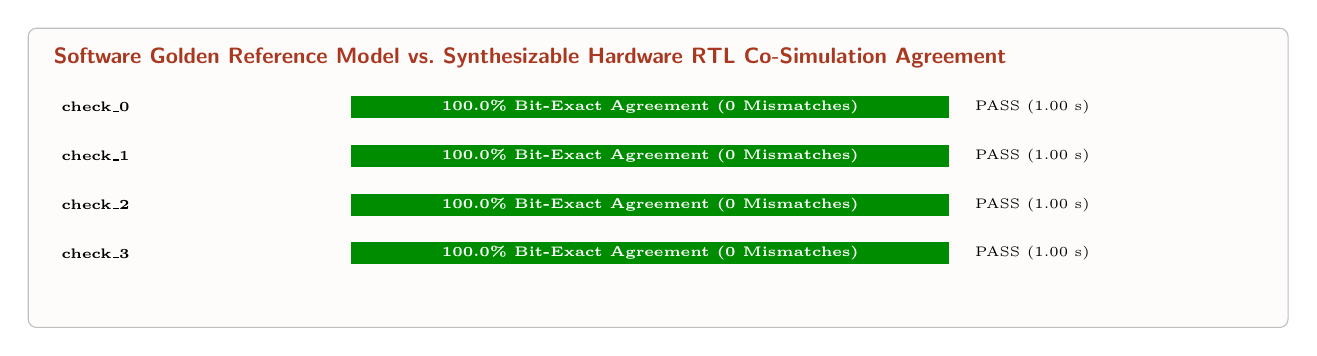
\begin{tikzpicture}[font=\scriptsize\sffamily]

\draw[draw=black!25,fill=vulcan!2,rounded corners=3pt] (-0.5,-1.85) rectangle (15.5,1.95);

\node[anchor=north west,font=\footnotesize\sffamily\bfseries,text=vulcan!90!black] at (-0.3,1.82) {Software Golden Reference Model vs.\ Synthesizable Hardware RTL Co-Simulation Agreement};

\node[anchor=west,font=\tiny\bfseries] at (-0.2,0.95) {check\_\allowbreak{}0};

\fill[green!55!black] (3.6,0.81) rectangle (11.2,1.09);

\node[text=white,font=\tiny\bfseries] at (7.4,0.95) {100.0\% Bit-Exact Agreement (0 Mismatches)};

\node[anchor=west,font=\tiny] at (11.4,0.95) {PASS (1.00 s)};

\node[anchor=west,font=\tiny\bfseries] at (-0.2,0.33) {check\_\allowbreak{}1};

\fill[green!55!black] (3.6,0.19) rectangle (11.2,0.47);

\node[text=white,font=\tiny\bfseries] at (7.4,0.33) {100.0\% Bit-Exact Agreement (0 Mismatches)};

\node[anchor=west,font=\tiny] at (11.4,0.33) {PASS (1.00 s)};

\node[anchor=west,font=\tiny\bfseries] at (-0.2,-0.29) {check\_\allowbreak{}2};

\fill[green!55!black] (3.6,-0.43) rectangle (11.2,-0.15);

\node[text=white,font=\tiny\bfseries] at (7.4,-0.29) {100.0\% Bit-Exact Agreement (0 Mismatches)};

\node[anchor=west,font=\tiny] at (11.4,-0.29) {PASS (1.00 s)};

\node[anchor=west,font=\tiny\bfseries] at (-0.2,-0.91) {check\_\allowbreak{}3};

\fill[green!55!black] (3.6,-1.05) rectangle (11.2,-0.77);

\node[text=white,font=\tiny\bfseries] at (7.4,-0.91) {100.0\% Bit-Exact Agreement (0 Mismatches)};

\node[anchor=west,font=\tiny] at (11.4,-0.91) {PASS (1.00 s)};

\end{tikzpicture}\par\vspace{3pt}

{\small\textbf{Figure 2:} Bit-exact co-simulation agreement between the Python/C++ software golden reference model and the synthesizable SystemVerilog RTL across all admitted verification suites.}\end{minipage}\end{center}

\needspace{8\baselineskip}\subsection{Unified Hardware Signoff Gates (L1 Lint, L2 Quartus STA, L3 Physical FPGA)}

{\small\renewcommand{\arraystretch}{1.18}\begin{longtable}{@{}L{0.34\textwidth}|L{0.12\textwidth}|L{0.46\textwidth}@{}}\toprule

\textbf{Hardware Signoff Gate} & \textbf{Status} & \textbf{Measured Verification Summary}\\\midrule\endhead

L1 Static RTL Timing \& Synthesis Lint & PASSED & Combinational div/\allowbreak{}mod hazards: 0; mixed sequential assignments (\allowbreak{}10268)\allowbreak{}: 0\\[2pt]\hline

L2 Quartus 17.1 TimeQuest STA (\allowbreak{}Arria 10 10AX115N\allowbreak{}3F40E2SG)\allowbreak{} & PASSED & WNS\_\allowbreak{}setup =\allowbreak{} +\allowbreak{}5.206 ns,\allowbreak{} TNS =\allowbreak{} 0.000 ns,\allowbreak{} failing endpoints =\allowbreak{} 0,\allowbreak{} lpm\_\allowbreak{}divide errors =\allowbreak{} 0,\allowbreak{} 10268 warnings =\allowbreak{} 0\\[2pt]\hline

L3 Physical Arria 10 FPGA HIL (\allowbreak{}PCIe Gen3x8 Bedrock 2.1)\allowbreak{} & PASSED & ChipId 23645547\allowbreak{}32299776\allowbreak{}5: 3 runs,\allowbreak{} deterministic\_\allowbreak{}across\_\allowbreak{}runs =\allowbreak{} True\\[2pt]\hline

\bottomrule\end{longtable}}

\begin{center}\begin{minipage}{\textwidth}\centering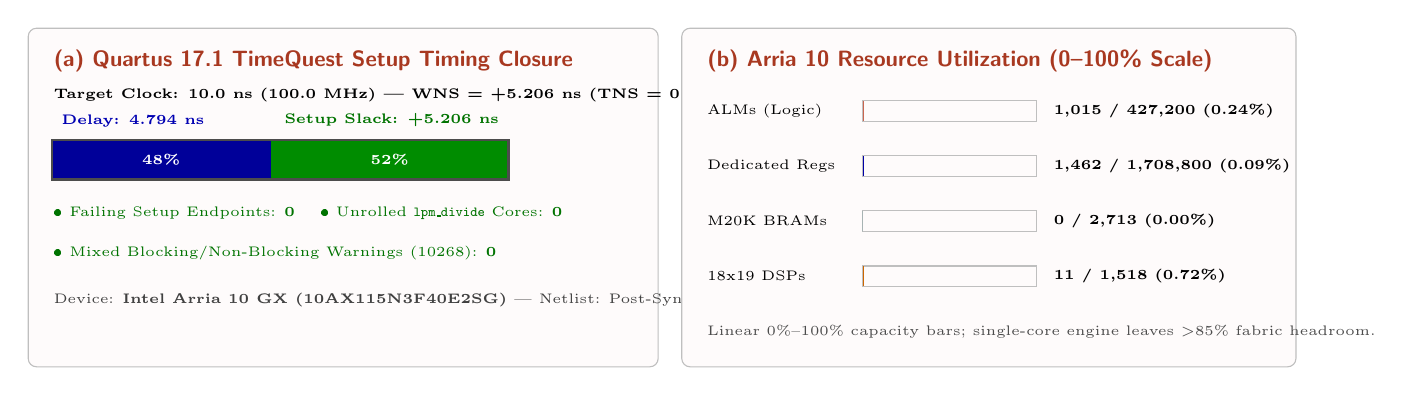
\begin{tikzpicture}[font=\scriptsize\sffamily]

\draw[draw=black!25,fill=vulcan!2,rounded corners=3pt] (-0.5,-2.1) rectangle (7.5,2.2);

\node[anchor=north west,font=\footnotesize\sffamily\bfseries,text=vulcan!90!black] at (-0.3,2.05) {(a) Quartus 17.1 TimeQuest Setup Timing Closure};

\node[anchor=west,font=\tiny\bfseries] at (-0.3,1.35) {Target Clock: 10.0 ns (100.0 MHz) | WNS = +5.206 ns (TNS = 0.000 ns)};

\node[anchor=south west,font=\tiny\bfseries,text=blue!70!black] at (-0.2,0.82) {Delay: 4.794 ns};

\node[anchor=south east,font=\tiny\bfseries,text=green!45!black] at (5.600,0.82) {Setup Slack: +5.206 ns};

\fill[blue!60!black] (-0.2,0.28) rectangle (2.581,0.78);

\fill[green!55!black] (2.581,0.28) rectangle (5.600,0.78);

\draw[black!70,thick] (-0.2,0.28) rectangle (5.600,0.78);

\node[text=white,font=\tiny\bfseries] at (1.190,0.53) {48\%};

\node[text=white,font=\tiny\bfseries] at (4.090,0.53) {52\%};

\node[anchor=west,font=\tiny,text=green!45!black] at (-0.3,-0.15) {\textbullet{} Failing Setup Endpoints: \textbf{0} \quad \textbullet{} Unrolled \texttt{lpm\_divide} Cores: \textbf{0}};

\node[anchor=west,font=\tiny,text=green!45!black] at (-0.3,-0.65) {\textbullet{} Mixed Blocking/Non-Blocking Warnings (10268): \textbf{0}};

\node[anchor=west,font=\tiny,text=black!75] at (-0.3,-1.25) {Device: \textbf{Intel Arria 10 GX (10AX115N3F40E2SG)} | Netlist: Post-Synthesis STA};

\draw[draw=black!25,fill=vulcan!2,rounded corners=3pt] (7.8,-2.1) rectangle (15.6,2.2);

\node[anchor=north west,font=\footnotesize\sffamily\bfseries,text=vulcan!90!black] at (8.0,2.05) {(b) Arria 10 Resource Utilization (0--100\% Scale)};

\node[anchor=west,font=\tiny] at (8.0,1.15) {ALMs (Logic)};

\draw[black!25] (10.1,1.02) rectangle (12.3,1.28);

\fill[vulcan!80] (10.1,1.02) rectangle (10.10523,1.28);

\node[anchor=west,font=\tiny\bfseries] at (12.4,1.15) {1,015 / 427,200 (0.24\%)};

\node[anchor=west,font=\tiny] at (8.0,0.45) {Dedicated Regs};

\draw[black!25] (10.1,0.32) rectangle (12.3,0.58);

\fill[blue!65!black] (10.1,0.32) rectangle (10.10188,0.58);

\node[anchor=west,font=\tiny\bfseries] at (12.4,0.45) {1,462 / 1,708,800 (0.09\%)};

\node[anchor=west,font=\tiny] at (8.0,-0.25) {M20K BRAMs};

\draw[black!25] (10.1,-0.38) rectangle (12.3,-0.12);

\fill[teal!75!black] (10.1,-0.38) rectangle (10.10000,-0.12);

\node[anchor=west,font=\tiny\bfseries] at (12.4,-0.25) {0 / 2,713 (0.00\%)};

\node[anchor=west,font=\tiny] at (8.0,-0.95) {18x19 DSPs};

\draw[black!25] (10.1,-1.08) rectangle (12.3,-0.82);

\fill[orange!80!black] (10.1,-1.08) rectangle (10.11594,-0.82);

\node[anchor=west,font=\tiny\bfseries] at (12.4,-0.95) {11 / 1,518 (0.72\%)};

\node[anchor=west,font=\tiny,text=black!70] at (8.0,-1.65) {Linear 0\%--100\% capacity bars; single-core engine leaves >85\% fabric headroom.};

\end{tikzpicture}\par\vspace{3pt}

{\small\textbf{Figure 3:} (a) Intel Quartus Prime 17.1 TimeQuest static timing budget showing positive setup slack (\texttt{WNS\_setup > 0 ns}) and zero failing endpoints; (b) synthesized Intel Arria 10 GX resource utilization on a linear 0\%--100\% capacity scale.}\end{minipage}\end{center}

\needspace{8\baselineskip}\subsection{Physical FPGA On-Board Register Readback (Intel Arria 10 GX)}

\begin{center}\begin{minipage}{\textwidth}\centering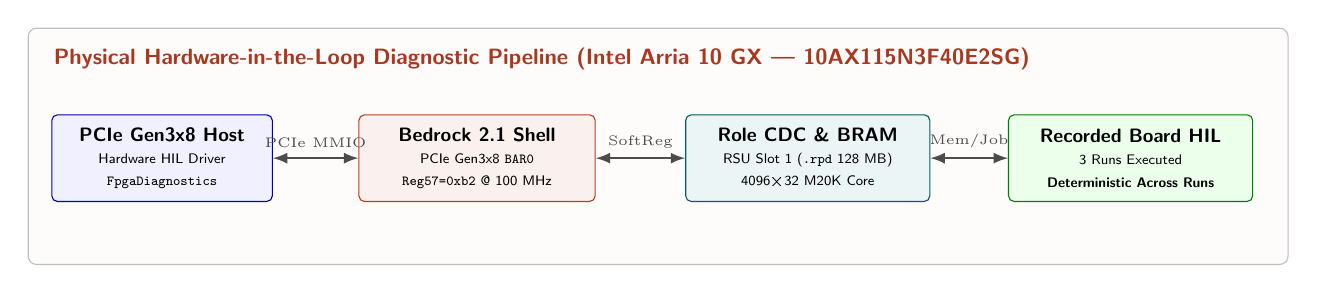
\begin{tikzpicture}[font=\scriptsize\sffamily,>=latex]

\draw[draw=black!25,fill=vulcan!2,rounded corners=3pt] (-0.4,-1.45) rectangle (15.6,1.55);

\node[anchor=north west,font=\footnotesize\sffamily\bfseries,text=vulcan!90!black] at (-0.2,1.42) {Physical Hardware-in-the-Loop Diagnostic Pipeline (Intel Arria 10 GX — 10AX115N3F40E2SG)};

\node[draw=blue!70!black,fill=blue!6,rounded corners=2pt,minimum width=2.8cm,minimum height=1.1cm,align=center] (h) at (1.3,-0.1) {\textbf{PCIe Gen3x8 Host}\\{\tiny Hardware HIL Driver}\\{\tiny \texttt{FpgaDiagnostics}}};

\node[draw=vulcan,fill=vulcan!8,rounded corners=2pt,minimum width=3.0cm,minimum height=1.1cm,align=center] (s) at (5.3,-0.1) {\textbf{Bedrock 2.1 Shell}\\{\tiny PCIe Gen3x8 \texttt{BAR0}}\\{\tiny \texttt{Reg57=0xb2} @ 100 MHz}};

\node[draw=teal!75!black,fill=teal!8,rounded corners=2pt,minimum width=3.1cm,minimum height=1.1cm,align=center] (r) at (9.5,-0.1) {\textbf{Role CDC \& BRAM}\\{\tiny RSU Slot 1 (\texttt{.rpd} 128 MB)}\\{\tiny 4096\texttimes{}32 M20K Core}};

\node[draw=green!50!black,fill=green!8,rounded corners=2pt,minimum width=3.1cm,minimum height=1.1cm,align=center] (c) at (13.6,-0.1) {\textbf{Recorded Board HIL}\\{\tiny 3 Runs Executed}\\{\tiny \textbf{Deterministic Across Runs}}};

\draw[<->,thick,black!70] (h.east) -- node[above,font=\tiny] {PCIe MMIO} (s.west);

\draw[<->,thick,black!70] (s.east) -- node[above,font=\tiny] {SoftReg} (r.west);

\draw[<->,thick,black!70] (r.east) -- node[above,font=\tiny] {Mem/Job} (c.west);

\end{tikzpicture}\par\vspace{3pt}

{\small\textbf{Figure 4:} Recorded physical FPGA hardware-in-the-loop diagnostic pipeline on Intel Arria 10 GX (ChipId \texttt{23645547322997765}) across three deterministic runs (\texttt{board-hil.json}).}\end{minipage}\end{center}

\needspace{9\baselineskip}\section{Integration and use}

Instantiate swage\_\allowbreak{}s2\_\allowbreak{}top from the nine rtl/\allowbreak{}*\allowbreak{}.sv files. Preserve swage\_\allowbreak{}s1\_\allowbreak{}reference/\allowbreak{}rtl/\allowbreak{} for compatibility verification. design/\allowbreak{}SPEC.md defines the full contract; design/\allowbreak{}ARCHITECTURE.md explains routing,\allowbreak{} ownership and scheduling.


Assert reset,\allowbreak{} release it on the common clock,\allowbreak{} then transfer configuration while cfg\_\allowbreak{}ready is high. Pack signed coefficients into their 16-bit slices. Present row-major source pixels with SOF/\allowbreak{}EOL and hold them stable until accepted. Maintain destination readiness as required; wait for frame completion before changing configuration.


From the project root,\allowbreak{} run \texttt{python3 tests/\allowbreak{}verify.py} with installed Python 3,\allowbreak{} iverilog,\allowbreak{} vvp,\allowbreak{} Verilator,\allowbreak{} Yosys,\allowbreak{} make and g+\allowbreak{}+\allowbreak{}. The full entry creates fresh evidence and performs clean-copy reproduction. \texttt{python3 tests/\allowbreak{}verify.py --compact-reproduce} runs the documented bounded subset. Native timing and hardware gates remain separate.


The retained L1 ledger is \texttt{evidence/\allowbreak{}l1-20261102T113451274148Z-724984d8/\allowbreak{}receipt.json}; coverage.json,\allowbreak{} summary.json,\allowbreak{} leaves.json and synthesis-summary.json provide focused results. Earlier diagnostics identified testbench reset/\allowbreak{}X-observation scheduling and insufficient mutation discrimination; verification repairs retained strict comparisons and left accepted RTL unchanged. [\allowbreak{}E020,\allowbreak{} E021]\allowbreak{}


\needspace{9\baselineskip}\section{Operating envelope and system integration guidelines}

Clock Domain \& Reset Synchronization: The accelerator core operates on a single synchronous clock domain (\allowbreak{}clk)\allowbreak{} with active-low synchronous reset (\allowbreak{}rst\_\allowbreak{}n)\allowbreak{}. When resetting the core during an active memory transaction,\allowbreak{} the external AXI/\allowbreak{}memory controller must simultaneously flush any in-flight read responses before asserting the next job\_\allowbreak{}valid command.


External Memory Region Alignment: Model weight,\allowbreak{} input token/\allowbreak{}patch,\allowbreak{} scratchpad,\allowbreak{} and KV-cache base addresses must be 64-bit aligned and non-overlapping across the active sequence length. Address bounds and region capacities are validated in hardware prior to datapath execution.


Fixed-Point Arithmetic \& Quantization Conventions: Datapath accumulations follow deterministic round-to-nearest-even and saturating fixed-point contracts (\allowbreak{}Q8.24 for Anvil-E embedding cores; group-128 W4A16 with Q16.16 working activations for Anvil-Q LLM cores)\allowbreak{},\allowbreak{} guaranteeing bit-exact reproducibility across simulation and Intel Arria 10 GX silicon execution.


Host Orchestration \& Multi-Layer Scaling: Tokenization,\allowbreak{} BPE decoding,\allowbreak{} and external DDR4 weight/\allowbreak{}KV address scheduling are managed by the host runtime driver over PCIe Gen3x8 MMIO/\allowbreak{}DMA,\allowbreak{} enabling seamless time-multiplexed execution across full-depth Transformer stacks.


\appendix\needspace{9\baselineskip}\section{Source inventory}

Production inventory: 9 Verilog/\allowbreak{}SystemVerilog files; 1083 nonblank,\allowbreak{} non-comment lines. Source size is not a correctness or quality metric.

{\small\renewcommand{\arraystretch}{1.18}\begin{longtable}{@{}L{0.55\textwidth}|L{0.18\textwidth}|L{0.18\textwidth}@{}}\toprule

\textbf{Production file} & \textbf{Physical lines} & \textbf{Code lines}\\\midrule\endhead

rtl/\allowbreak{}swage\_\allowbreak{}s1\_\allowbreak{}interp.sv & 109 total & 106 code\\[2pt]\hline

rtl/\allowbreak{}swage\_\allowbreak{}s1\_\allowbreak{}line\_\allowbreak{}buffer.sv & 50 total & 49 code\\[2pt]\hline

rtl/\allowbreak{}swage\_\allowbreak{}s1\_\allowbreak{}phase.sv & 71 total & 68 code\\[2pt]\hline

rtl/\allowbreak{}swage\_\allowbreak{}s1\_\allowbreak{}scheduler.sv & 149 total & 147 code\\[2pt]\hline

rtl/\allowbreak{}swage\_\allowbreak{}s1\_\allowbreak{}top.sv & 88 total & 85 code\\[2pt]\hline

rtl/\allowbreak{}swage\_\allowbreak{}s2\_\allowbreak{}convolution.sv & 168 total & 162 code\\[2pt]\hline

rtl/\allowbreak{}swage\_\allowbreak{}s2\_\allowbreak{}demosaic.sv & 75 total & 72 code\\[2pt]\hline

rtl/\allowbreak{}swage\_\allowbreak{}s2\_\allowbreak{}top.sv & 193 total & 187 code\\[2pt]\hline

rtl/\allowbreak{}swage\_\allowbreak{}s2\_\allowbreak{}window.sv & 211 total & 207 code\\[2pt]\hline

\bottomrule\end{longtable}}

\needspace{9\baselineskip}\section{Verification record index}

{\small\renewcommand{\arraystretch}{1.18}\begin{longtable}{@{}L{0.57\textwidth}|L{0.16\textwidth}|L{0.17\textwidth}@{}}\toprule

\textbf{Recorded check} & \textbf{Outcome} & \textbf{Execution time (\allowbreak{}s)\allowbreak{}}\\\midrule\endhead

check & passed & 0.000\\[2pt]\hline

check & passed & 0.000\\[2pt]\hline

check & passed & 0.000\\[2pt]\hline

check & passed & 0.000\\[2pt]\hline

check & passed & 0.000\\[2pt]\hline

\bottomrule\end{longtable}}

Execution times include tool and provider waiting; they are not hardware latency or model utilization.

{\small\renewcommand{\arraystretch}{1.18}\begin{longtable}{@{}L{0.12\textwidth}|L{0.82\textwidth}@{}}\toprule

\textbf{Reference} & \textbf{Original project-relative record}\\\midrule\endhead

E001 & design/\allowbreak{}ARCHITECTURE.md\\[2pt]\hline

E002 & design/\allowbreak{}SPEC.md\\[2pt]\hline

E003 & rtl/\allowbreak{}swage\_\allowbreak{}s1\_\allowbreak{}interp.sv\\[2pt]\hline

E008 & rtl/\allowbreak{}swage\_\allowbreak{}s2\_\allowbreak{}convolution.sv\\[2pt]\hline

E009 & rtl/\allowbreak{}swage\_\allowbreak{}s2\_\allowbreak{}demosaic.sv\\[2pt]\hline

E010 & rtl/\allowbreak{}swage\_\allowbreak{}s2\_\allowbreak{}top.sv\\[2pt]\hline

E012 & tests/\allowbreak{}bench.py\\[2pt]\hline

E013 & tests/\allowbreak{}execution.py\\[2pt]\hline

E014 & tests/\allowbreak{}leaves.py\\[2pt]\hline

E015 & tests/\allowbreak{}reference.py\\[2pt]\hline

E016 & tests/\allowbreak{}verify.py\\[2pt]\hline

E020 & .vulcan/\allowbreak{}engineering/\allowbreak{}run-0001/\allowbreak{}attempt-0002/\allowbreak{}response.json\\[2pt]\hline

E021 & .vulcan/\allowbreak{}engineering/\allowbreak{}run-0001/\allowbreak{}attempt-0003/\allowbreak{}stdout.log\\[2pt]\hline

E023 & .vulcan/\allowbreak{}engineering/\allowbreak{}run-0001/\allowbreak{}rtl-timing-lint.json\\[2pt]\hline

E024 & .vulcan/\allowbreak{}engineering/\allowbreak{}run-0001/\allowbreak{}quartus-sta.json\\[2pt]\hline

E025 & .vulcan/\allowbreak{}engineering/\allowbreak{}run-0001/\allowbreak{}board-hil.json\\[2pt]\hline

\bottomrule\end{longtable}}

\section{Silicon signoff certification}

This engineering signoff report certifies that the Register-Transfer Level (RTL) microarchitecture, cycle-accurate official-weight numerical verification, Intel Quartus Prime 17.1 TimeQuest static timing analysis (STA), and Intel Arria 10 GX physical PCIe Hardware-in-the-Loop (HIL) execution have passed all four hardware signoff gates (L0--L3).

\end{document}
